In this chapter, we review the main challenges of denoising \gls{MPES} data, to enhance the interpretability of experimental results obtained from low-count datasets. We begin with exploring the various \gls{MPES} datasets used in this study, which include \gls{GrIr}, \gls{NiW}, \gls{GdW} and \gls{WSe2}, focusing on their characteristics relevant to analyzing the denoising performance.

An overview of the data reduction and image formation pipeline is provided, illustrating how single-event data from these experiments are transformed into multidimensional images suitable for analysis. We detail how the target and noisy realizations of the data are constructed, generating representations for high-count reference images and low-count noisy images that reflect realistic experimental conditions, respectively.

In order to evaluate the performance of denoising algorithms on \gls{MPES} data, we present here the criteria and metrics used; in particular, focusing on perceptual metrics like the \gls{MSSSIM} (\cref{eq:msssim})\todo[disable]{Insert a reference to where you define this.}, which is more robust to the inherent noise in experimental reference images.

We apply the \gls{BM3D} algorithm, both with and without application of the Anscombe \gls{VST}, to the datasets. A hyperparameter search is performed to identify the optimal denoising parameters, specifically the choice of the $\sigma$ value, for different total electron counts  \gls{ncounts}. An evaluation of the denoising performance using the \gls{BM3D} algorithm on one \todo{By saying that you do this one ``one'' of the data sets, you implicitly stress that you don't do it on all, so the reader will wonder why. Depending on why you only do this on one dataset, you could make this clear by adding some clarification, i.e., just the ``exemplarily'' could be enough.} of the \gls{MPES} datasets is then demonstrated, with a discussion on the effectiveness of \gls{BM3D} in improving image quality at various count levels and the effect of applying \gls{VST} on denoising performance.

\section{Experimental Datasets}\label{section:datasets}
We investigate three datasets--\gls{GrIr} \cite{heberMultispectralTimeresolvedEnergy2022}, \gls{NiW} \cite{shokeenRealtimeObservationNonequilibrium2024}, and \gls{GdW} \cite{kutnyakhovMultidimensionalPhotoemissionSpectra2024}--that have been studied using \gls{HEXTOF} at \gls{FLASH}. Interpretable results from these experiments require long acquisition times (\gls{total_time}), essential for capturing the underlying physical processes. This is primarily due to three reasons discussed earlier:\todo[disable]{``that will be described below''?}.

\todo[disable]{You could reference the corresponding section here}The intrinsic stochastic nature of the photoemission process requires the collection of a large number of events to approach the true value (\cref{section:photoemission-process}). Additionally, the low repetition rate and intentionally reduced flux\footnote{To mitigate the space-charge effect} of the \gls{FEL} means that the data  needs to be collected over a long period of time to get sufficient statistics (\cref{section:fel}). For example, as shown in \cref{fig:acq-time-1M}, acquiring $\num{e6}$ electron events (\gls{ncounts}) \todo[disable]{electrons? events?} requires an acquisition time of $\gls{total_time}=\qty{8}{\min}$. Lastly, the multidimensional acquisition scheme to simultaneously resolve \gls{kx}, \gls{ky}, \gls{kz}, \gls{E}, \gls{tpp}, and spin polarization necessitates exponentially \todo[disable]{You mean this scale exponentially in the number od dimensions?} more data, as the number of dimensions increases, to adequately fill the sample space in higher dimensions (\cref{section:spectroscopy-techniques}).

\begin{figure}[h]
    \centering
    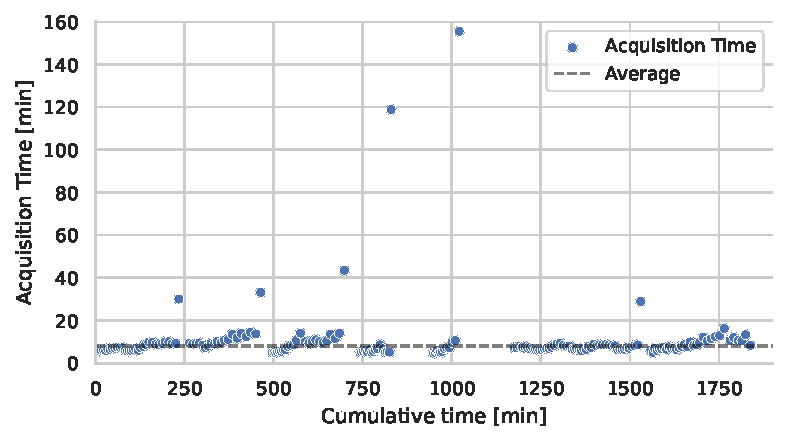
\includegraphics[width=0.8\linewidth]{images/acq_time_1M.pdf}
    \caption{Total acquisition time \gls{total_time} in minutes for generating \num{e6} data points. Some outliers are present due to the photon source being off, leading to longer \gls{total_time}. The average \gls{total_time} without outliers is approximately \qty{8}{min} (see dashed line).}
    \label{fig:acq-time-1M}
\end{figure}

For most of this study, we use the \gls{GrIr} dataset, as it features the longest acquisition time $T=\qty{30}{h}$, and hence the highest number of counts, with $\gls{ncounts}=\num{1.86e8}$\todo[disable]{You may also want to (re-)state $T$ for this data set here.}. The \gls{NiW} and \gls{GdW} datasets have comparatively lower total counts, at $\gls{ncounts}$ of \num{6.52e7} and \num{2.21e7}, respectively. 

However, \gls{ncounts} is not the only factor in determining data quality. Material-specific factors, sample conditions, and instrument settings can influence spectral clarity, meaning that a higher-count dataset does not necessarily guarantee more pronounced spectral features. For instance, while the \gls{NiW} dataset has higher counts \todo[disable]{Why ``\gls{ncounts}''? Isn't this the number of counts that you are referring to? I would interpret ``rate'' as counts per time, but you seem to give the absolute counts here.}\tododone[disable]{Yes, just by mistake} than \gls{GdW}, its spectral features are comparatively less distinct as seen in \cref{fig:all-hextof-datasets-kxky}.

\begin{figure}[h]
    \centering
    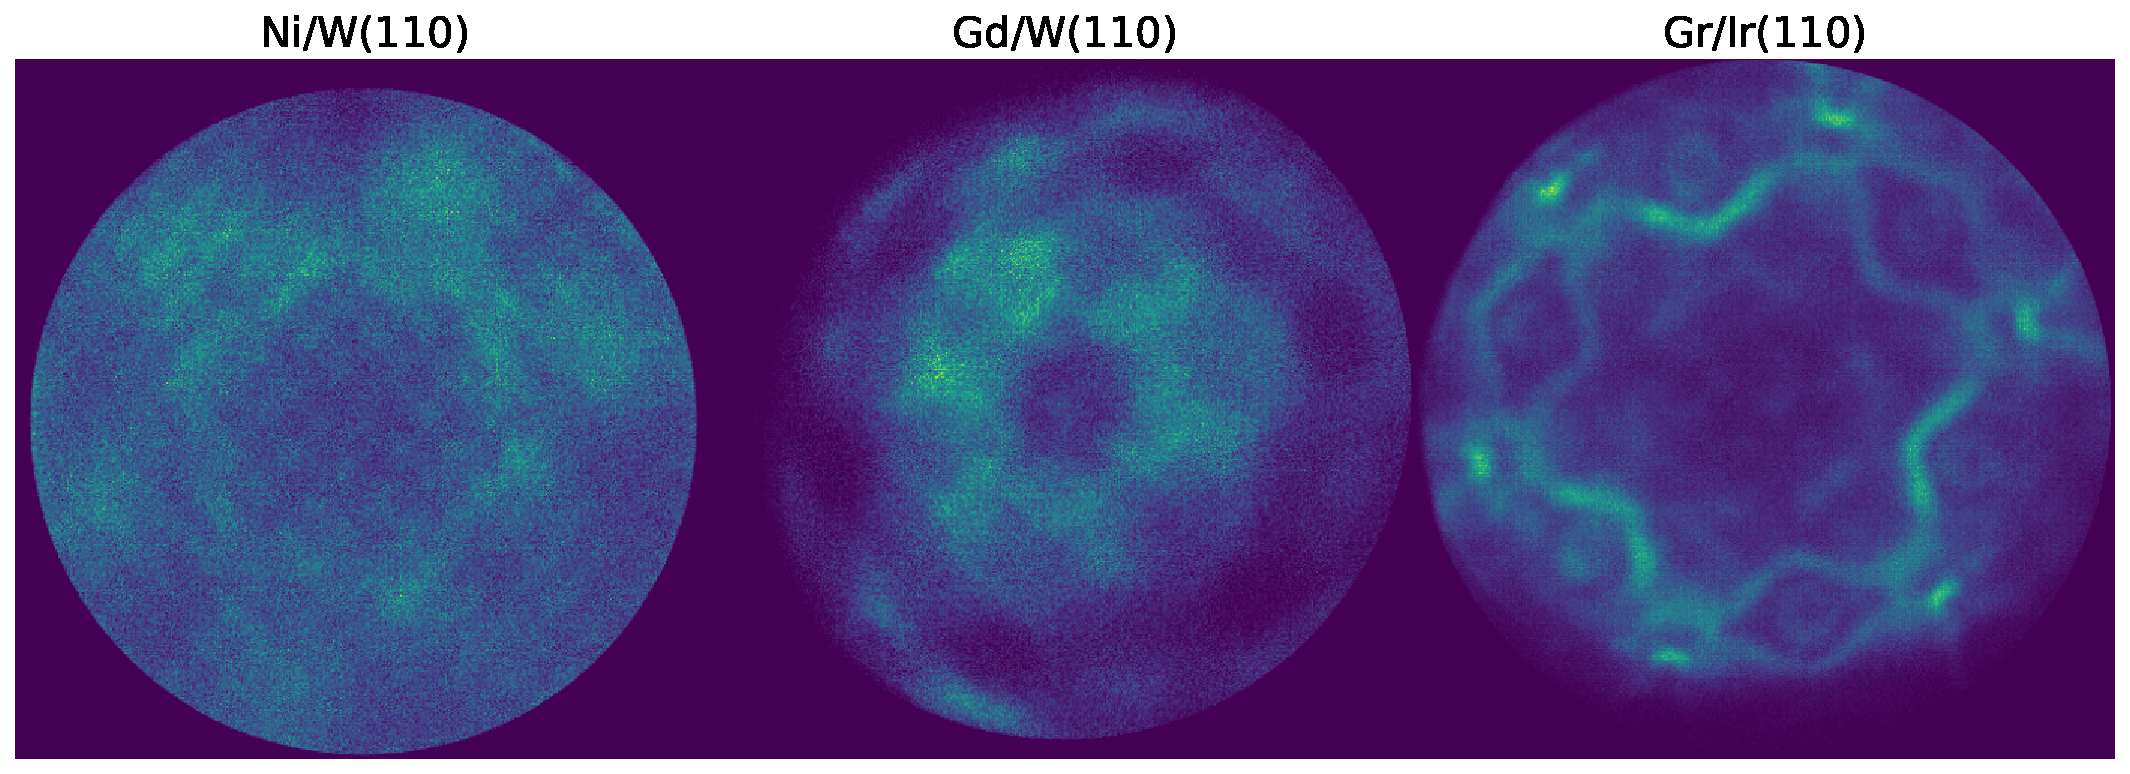
\includegraphics[width=1\linewidth]{images/datasets_3_kx_ky.pdf}
    \caption{A \gls{kx}-\gls{ky} slice of the \gls{GrIr}, \gls{NiW}, and \gls{GdW} datasets, window-averaged across \gls{E} with window size \todo[disable]{insert ``window size''}$\gls{winsize}=\num{20}$\todo[disable]{Is the size in ``bins''? I guess what this means will only become clear in Section 4.2. If this is the case, you also can reference this here, so the reader will know to look for the details furher down.}. See \cref{sec:image-formation} for details on how these images are formed.}
    \label{fig:all-hextof-datasets-kxky}
\end{figure}

For reference, we also look at the \gls{WSe2} dataset \cite{maklarTimeresolvedARPESRAW2022}, measured with a pulsed \gls{HHG}-based \gls{XUV} source using a \gls{TOF}-\gls{MM} analyzer\footnote{The \gls{TOF}-\gls{MM} analyzer being the common aspect between the \gls{GrIr} etc./ and the \gls{WSe2} dataset.} and a single-segmented \gls{DLD}. This setup yields a significantly larger number of counts, recording $\gls{ncounts}=\num{1e9}$ within $\gls{total_time}=\qty{27}{s}$. In comparison, the \gls{GrIr} dataset, collected with a \gls{FEL} source, yields $\gls{ncounts} = \num{1e6}$ over $\gls{total_time} = \qty{8}{\min}$, thus producing about four orders of magnitude fewer events.

A direct denoising comparison between these datasets, however, is not feasible due to fundamental differences in light sources and detector design. The \gls{WSe2} dataset was acquired with a single-segmented detector setup, whereas the \gls{GrIr} dataset employed a more complex 8-segment detector (\cref{section:8q-dld}) that offers enhanced multi-hit capability through overlapping segments, but impacting count statistics. This already implies that the finding equivalent noise levels between the datasets is a non-trivial task.

Additionally, the inherent statistical properties of the light sources (\cref{section:light-sources}) impact the noise characteristics in the raw data. Consequently, in \cref{ch:pes-statistics}, the \gls{WSe2} dataset aids in understanding statistical differences between acquisition setups. However, direct denoising comparisons between \gls{HHG} and \gls{FEL} sources would not be meaningful due to these varied conditions and detector architectures.

\section{Data Processing and Image Formation}\label{sec:image-formation}

In an \gls{MPES} experiment using a \gls{TOF}-based scheme, the workflow to resolve images typically follows a series of steps, outlined in \cref{fig:mpes_workflow}. Prior to this, an essential step is data reduction, a detailed description\footnote{More specific to the \gls{HEXTOF} instrument at \gls{FLASH}.} of which is outlined in Appendix~\ref{sec:elt}.

After the data reduction, corrections are applied to the measurement axes \todo[disable]{Minor cosmetic remark: Since you are not using \texttt{frenchspacing}, there is a double space after a ``.'' to mark the end of a sentence. This will also put such a double space after things like ``e.g.'' so it will look like an end of a sentence, even if it is not. One way to fix that would be to put a comma (before and) after ``e.g.'', i.e. ``, e.g.,''. Another way would be to put a backslash in front of the space after the ``.''. As I said though, this is a minor cosmetic issue, you can just ignore it if you want.} e.g.\ to correct space-charge distortions (see \cref{section:spectroscopy-techniques}), correct timing jitter between \gls{FEL} and pump laser etc. The corrected axes are then mapped (calibrated) to the physical axes, after which further correction steps can happen. Once calibrated, the single-event data is binned into a multidimensional volume\footnote{We make use of the Single Event DataFrame (SED) library \href{https://github.com/OpenCOMPES/sed}{https://github.com/OpenCOMPES/sed}.} that represents the full measurement, as illustrated on the right side of \cref{fig:mpes_workflow}.

\begin{figure}[h]
    \centering
    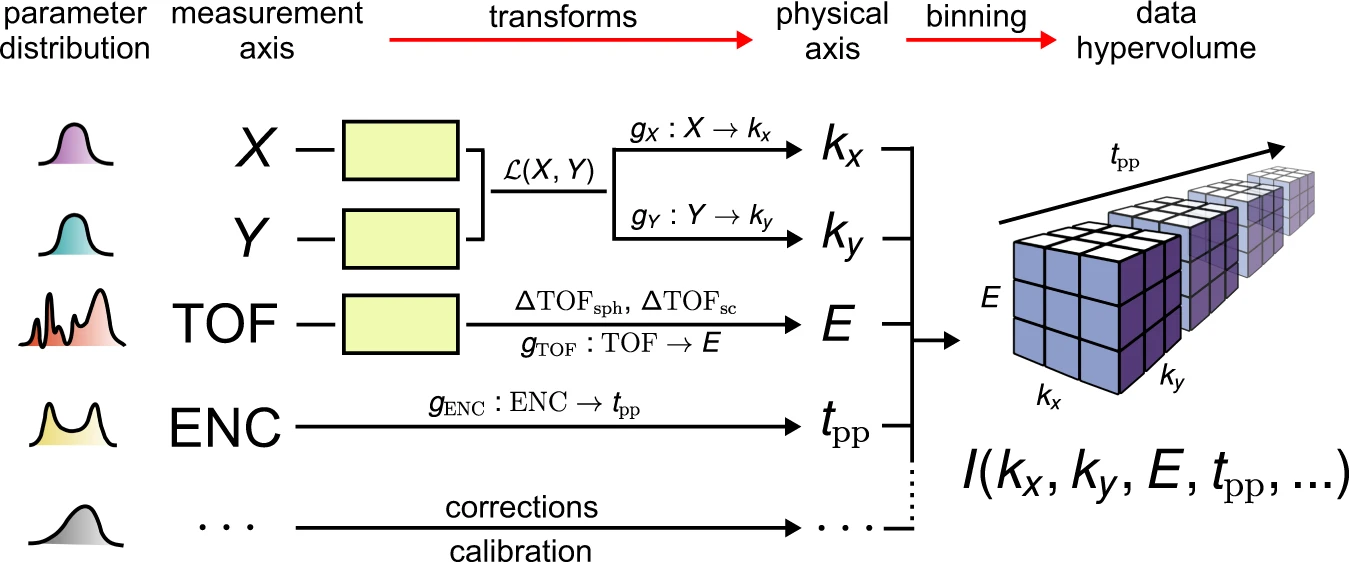
\includegraphics[width=1\linewidth]{images/41597_2020_769_Fig2_HTML.png}
    \caption{A typical workflow for an \gls{MPES} experiment, comprising transformations to the measured data and binning to form the multidimensional image. Reprinted from \cite{xianOpensourceEndtoendWorkflow2020}, under the terms of the Creative Commons Attribution 4.0 International License.}
    \label{fig:mpes_workflow}
\end{figure}

\subsection{Constructing Images from Single-Event Data}
% In \cref{eq:images}, we defined a $d$-dimensional latent clean image $Y$ and noisy image $X$. Let us define how these images are formed from event data. 

Let us take a look at the static (at equilibrium) spectra of the \gls{GrIr} dataset. That would mean aggregating (binning) data across the three detector axes\footnote{Reader is referred to \cref{section:dld} for details regarding detection scheme.}: $x$, $y$ and $t_{\text{tof}}$, corresponding to the physical axes \gls{kx}, \gls{ky} and \gls{E}, respectively. Binning these three axes forms a 3D \gls{kx}--\gls{ky}--\gls{E} image, as depicted in \cref{fig:3d-gr-ir}, comprising energy values both above and below the Fermi level \gls{EF}. \todo[disable]{I don't understand what focussing on a region means. As far as I understand, on of the dimensions of the 3D volume is still $E$.}

In this image, spatial dimensions ($x$ and $y$ directions) are binned with a resolution of \qty{460}{px}, corresponding to the native detector quantization. The $t_{\text{tof}}$ is also binned with \num{460} steps to match the spatial resolution\footnote{This is done to easily form equal-resolution 2D cuts across any dimension.}. Where the spatial dimensions ($x$ and $y$) are linearly mapped to the physical axes (\gls{kx}, \gls{ky}), the $E$ axis has a non-linear scaling with $t_{\text{tof}}$, making the $t_{\text{tof}}$ bins non-uniform in size when mapped to the $E$ axis. Hence, whenever we refer to binning of the $E$ axis, we are referring to binning along the $t_{\text{tof}}$ axis.

It is often useful to bin the data at a coarser granularity than the detector's native resolution, mainly to address low-count statistics, producing a representation that has lower resolution but higher count statistics. Coarse binning can be applied to a single dimension or across multiple dimensions. For instance, \cref{fig:all-hextof-datasets-kxky} showed 2D \gls{kx}--\gls{ky} images formed by window-averaging a region along the $E$ axis. This is effectively the same as coarsely binning the $E$ axis, and selecting a single slice from this coarser 3D image. Throughout this text, we use the native detector resolution as the baseline, and for coarser analyses, we specify the window size, \gls{winsize}, to define the averaging applied along a certain dimension. \todo[disable]{But this one uses additional averaging, doesn't it? Should also be mentioned here.}

While the full dataset contains \num{1.86e8} electron counts, the selected energy region used to generate the image in \cref{fig:3d-gr-ir-186M} contains \num{1.15e8} counts. Note that the energy range of interest is typically filtered, as not all detected energies are relevant for the analysis. Additionally, as discussed in \cref{section:8q-dld}, the majority of events are counted multiple times, with the most common case being that each event is recorded twice. This suggests that the effective number of counts is approximately half of \num{1.15e8}, i.e.\ \num{5.75e7}. For consistency, \gls{ncounts} is always referring to the total dataset count (\num{1.86e8} in this case), even if the actual unique counts may be lower due to multiple counting of events, or due to filtering of the energy range.

\begin{figure}
    \centering
    \begin{subfigure}[t]{0.49\linewidth}
        \centering
        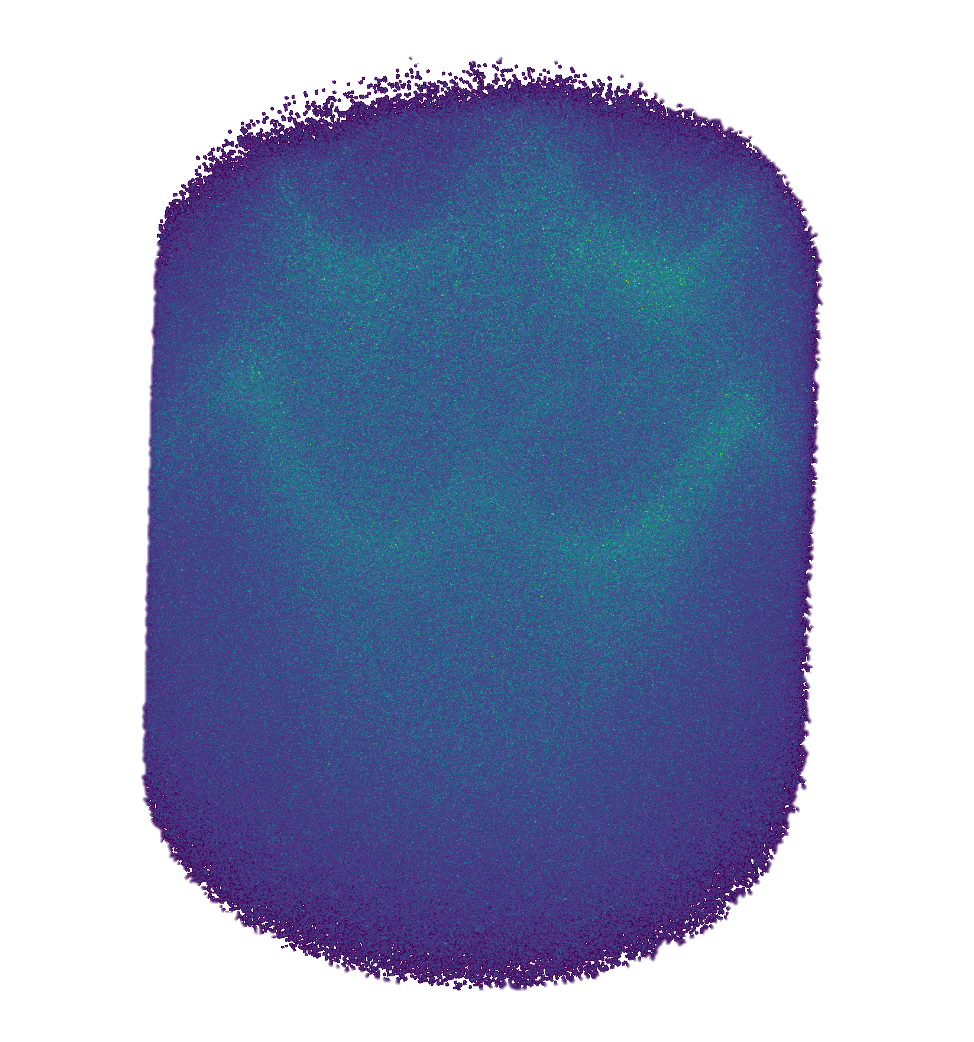
\includegraphics[width=1\linewidth]{images/3d_gr_ir_8M.png}
        \caption{$\gls{ncounts}=\num{8e6}$ corresponding to $\gls{total_time}=\qty{8}{min}$. The fine features of the data are not visible due to the low \gls{ncounts}.\todo[disable]{Do you really mean the ``rate'' (which you don't seem to specify) of the number of counts?}}
        \label{fig:3d-gr-ir-8M}
    \end{subfigure}
    \hfill
    \begin{subfigure}[t]{0.49\linewidth}
        \centering
        \includegraphics[width=1\linewidth]{images/3d_gr_ir_masked.png}
        \caption{$\gls{ncounts}=\num{1.86e8}$ corresponding to $\gls{total_time}=\qty{30}{hour}$. 2D images can be formed by slicing (or window-averaging) along any of the axes, as depicted by the three lines.}
        \label{fig:3d-gr-ir-186M}
    \end{subfigure}
    \caption{3D images from the \gls{GrIr} dataset, with $\gls{ncounts}=\num{8e6}$ (left) \todo[disable]{insert ``(left)''} and \num{1.86e8} (right)\todo[disable]{insert ``(right)''}. The image is constructed by binning over the three physical axes $k_x$, $k_y$, $E$.}
    \label{fig:3d-gr-ir}
\end{figure}

\subsection{Generation of Noisy Realizations}
With the \gls{DLD} providing a stream of single-event data, we are uniquely positioned to observe noisy realizations by taking subsets of varying electron counts \gls{ncounts} from the full dataset. These subsets can then be binned to form independent 3D images, used later for evaluating and training denoising algorithms.

For instance, from the complete dataset, \num{186} \todo{If you have a specif number here, I guess you mean also a specific data set. Which one is it? Due to this number, I guess \gls{GrIr}. And why 186? This looks like total number of counts divided by $10^6$, so you have data sets non-overlapping in time? Please make this clear in the text.} subsets, each with an \gls{ncounts} of \num{e6}, can be extracted. The data generation is assumed to be an \gls{iid} stochastic process, allowing for a large variety of randomly sampled subsets. However, due to the light source, which is not stable over extended periods, beyond its intrinsic fluctuations, sample degradation, temperature deviations and other reasons, this assumption is not entirely accurate.

\begin{table}[h!]
    \centering
    \resizebox{0.6\textwidth}{!}
        {%
        \begin{tabular}{lrrr}
            \toprule
            & \gls{ncounts} & Average Counts & $T$ [h] \\
            &  & Per Voxel & \\
            \midrule
            $n$ & \num{1e6} & \num{5.98e-3} & $\num{0.13}$ \\
            $2n$ & \num{2e6} & \num{1.22e-2} & $\num{0.28}$ \\
            $4n$ & \num{4e6} & \num{2.44e-2} & $\num{0.57}$ \\
            $8n$ & \num{8e6} & \num{4.89e-2} & $\num{1.23}$ \\
            $16n$ & \num{1.6e7} & \num{9.77e-2} & $\num{2.62}$ \\
            $32n$ & \num{3.2e7} & \num{2.00e-1} & $\num{5.32}$ \\
            $48n$ & \num{4.8e7} & \num{2.90e-1} & $\num{8.14}$ \\
            $96n$ & \num{9.6e7} & \num{5.84e-1} & $\num{16.07}$ \\
            $186n$ & \num{1.86e8} & \num{11.3e-1} & $\num{30.78}$ \\
            \bottomrule
        \end{tabular}
        }
    \caption{Table shows the noisy realizations generated by varying number of counts \gls{ncounts} from the \gls{GrIr} dataset. The acquisition time is proportional to \gls{ncounts} and $186n$ is used as the reference dataset.\todo[inline]{Just looking at this table and the text of Section 4.2.2, the $n$ column on the very left looks superfluous.}}
    \label{noisy-dataset-table}
\end{table}

Noisy realizations can then be formed based on different \gls{ncounts}. The total counts and average counts per voxel for each noisy realization are shown in \cref{noisy-dataset-table}. These realizations can help evaluate the performance of denoising algorithms as a function of \gls{total_time}. Lower count realizations ($\gls{ncounts}<\num{1e7}$), corresponding to shorter \gls{total_time}, are of most interest to denoise. Successful denoising of such data (such as image seen in \cref{fig:3d-gr-ir-8M}) could significantly improve experimental efficiency, allowing the investigators to steer the experiment in the right direction, crucial in time-limited \glspl{beamtime}. Hence, the realizations are sampled to cover a wide range of \gls{ncounts}, between \numrange{1e6}{1.86e8}.

\section{Evaluation Criteria}
As described in the last section, a 3D image is constructed by binning over the three physical axes $k_x$, $k_y$, $E$ from different datasets. By slicing along these axes, different 2D images can be generated for analysis. We evaluate the \gls{BM3D} algorithm, with and without the Anscombe transform\footnote{This was discussed in detail in \cref{ch:denoising}.}, using the \gls{GrIr} dataset, which has the highest average counts of all datasets. Despite this, the average voxel intensity is low (refer to \cref{noisy-dataset-table}), making a true, noise-free image unavailable. This limitation complicates the task of evaluating denoising performance, as standard metrics rely on comparison with such a noise-free reference.

Image quality assessment (IQA) is a field dedicated to measuring the objective and perpetual quality of an image. Objective metrics such as \gls{PSNR}, \gls{SSIM}, \gls{MSE} and \gls{MSSSIM} require a reference image\footnote{The metric definitions can be accessed in \cref{sec:metrics}.}---the latent clean image---to compare the denoised image against. No-reference metrics also exist, such as natural image quality evaluator (NIQE). However, these metrics are designed for real-world, non-scientific images. Subjective metrics such as the mean opinion score (MOS) can also be used, but these require evaluations by a group of experts, which can be impractical \cite{eskiciogluImageQualityMeasures1995,linzhangFSIMFeatureSimilarity2011}.

\begin{figure}
    \centering
    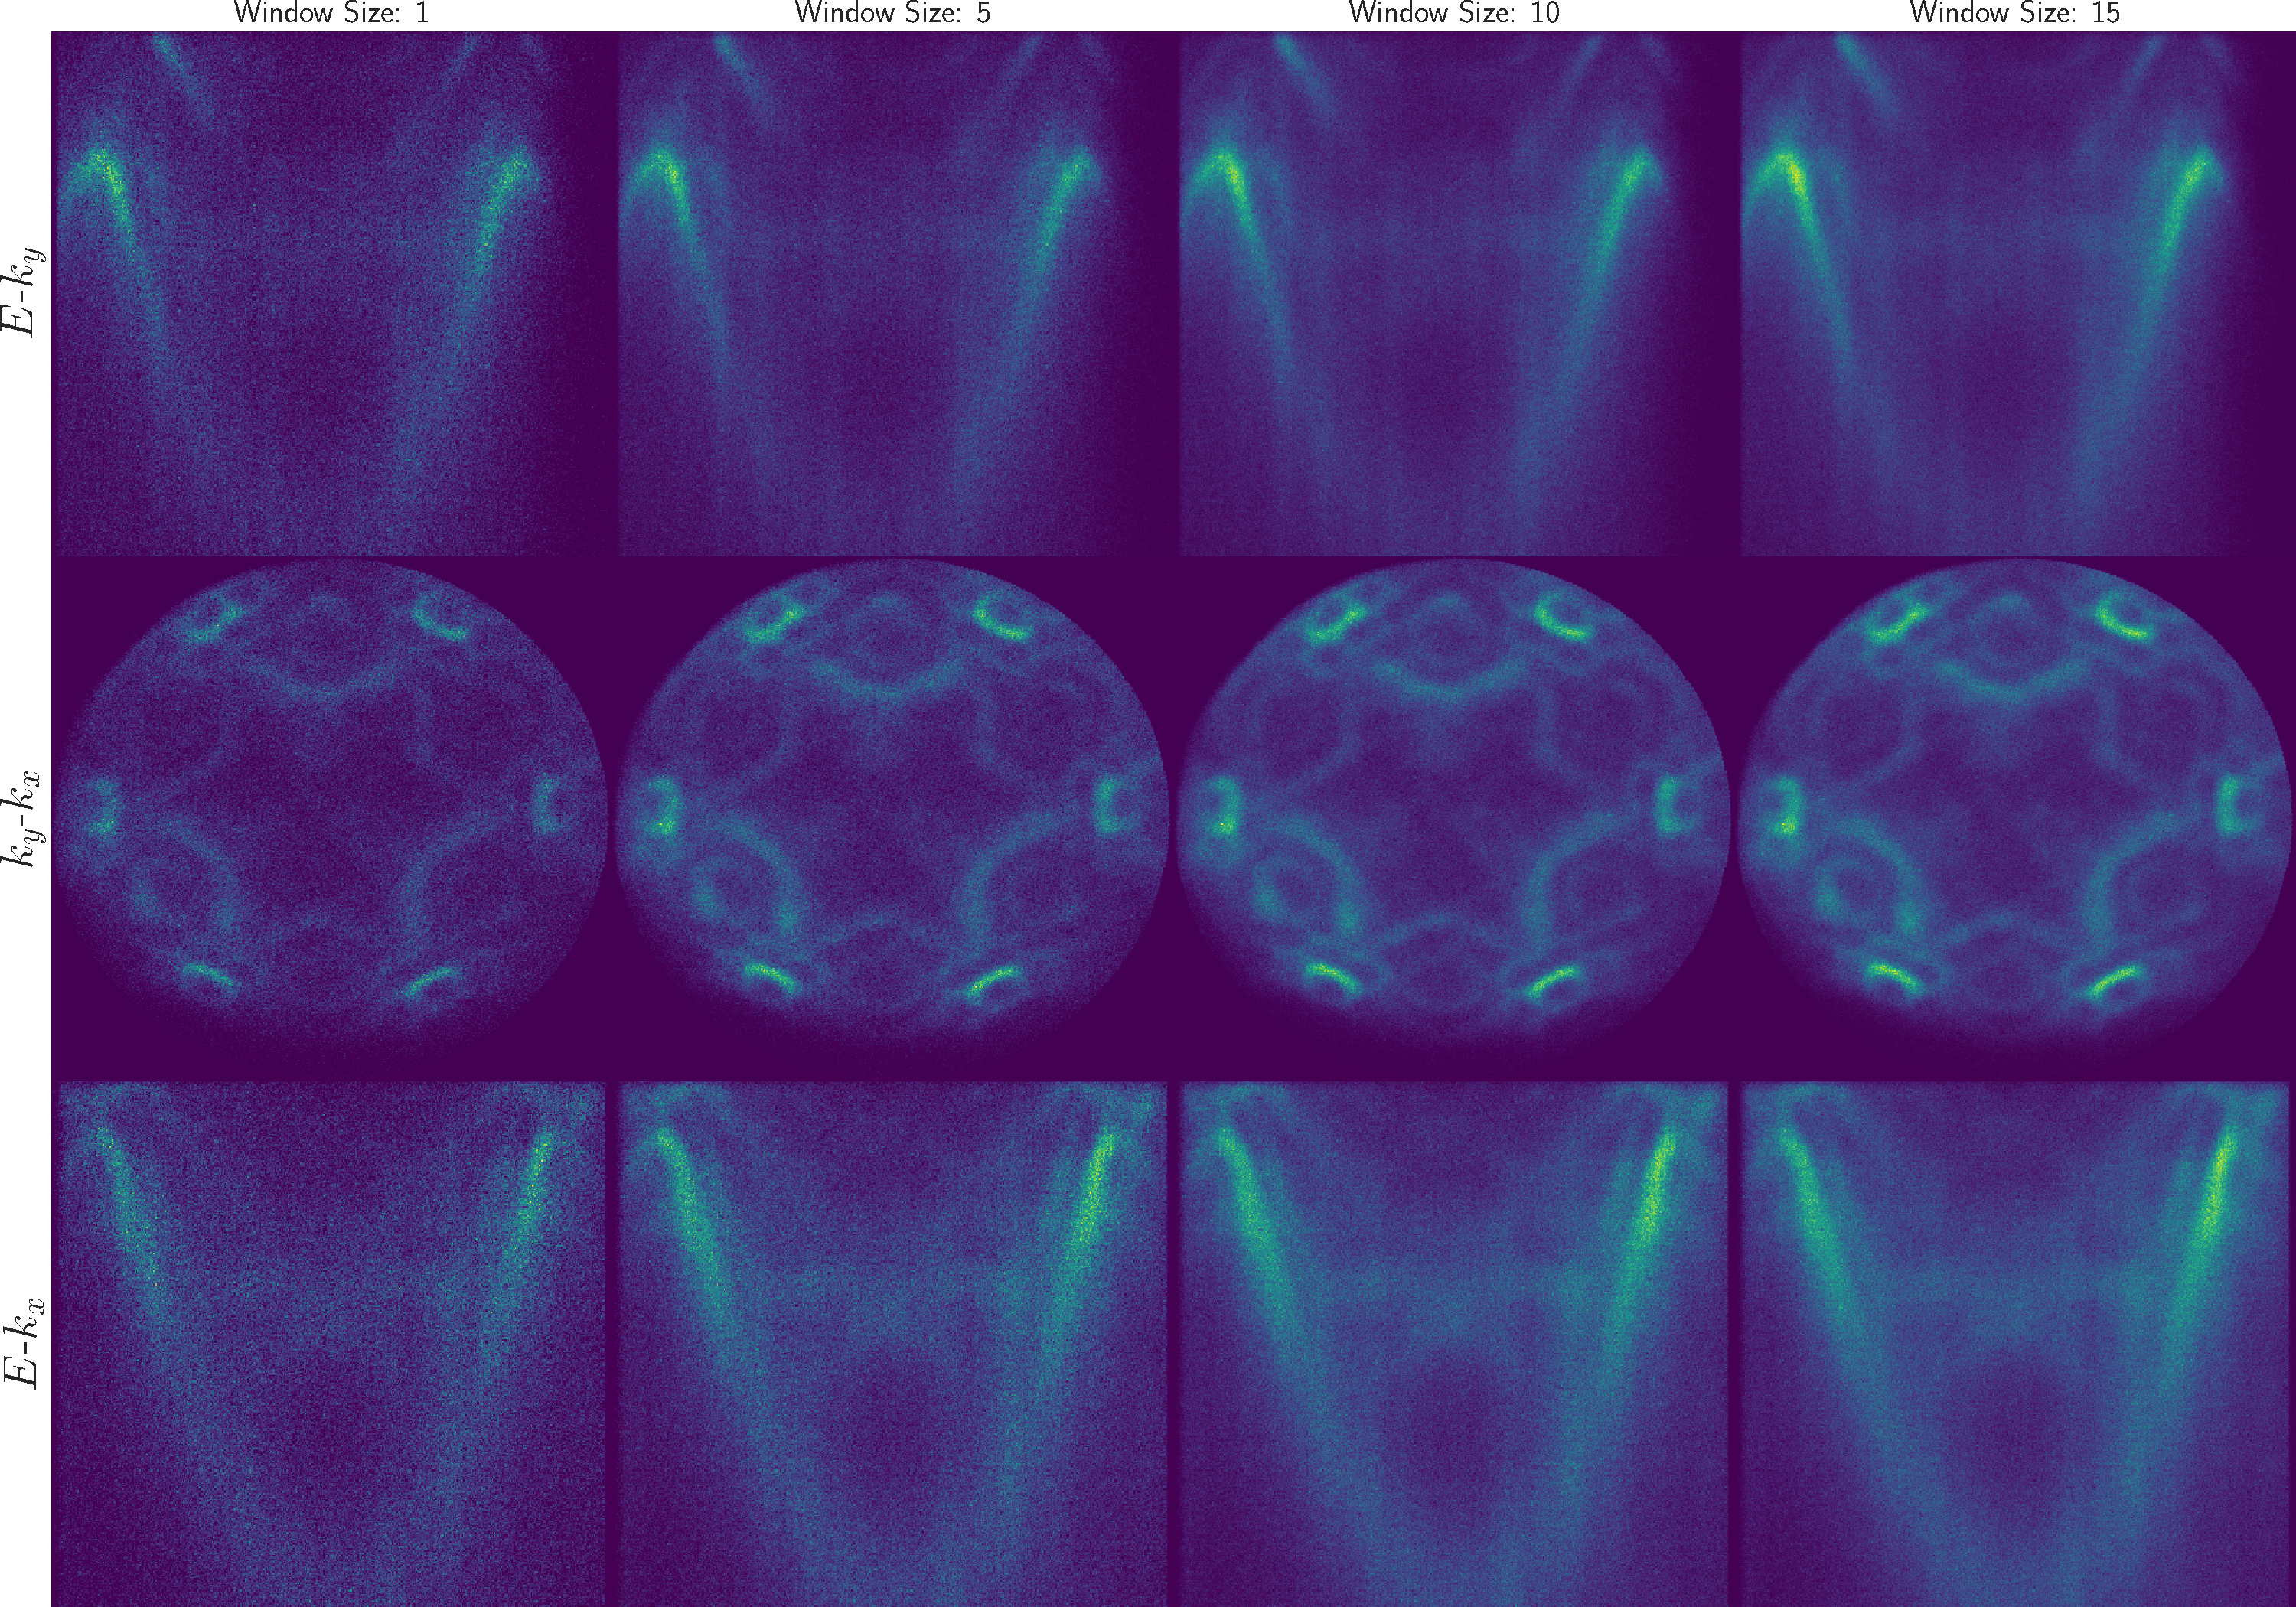
\includegraphics[width=1\linewidth]{images/slices.pdf}
    \caption{$E$, $k_y$, and $k_x$ slices at arbitrary positions of the \gls{GrIr} 3D dataset, showing the effect of averaging across different window sizes \gls{winsize}. The left most column shows a single slice ($\gls{winsize}=1$) with significant noise, while subsequent columns show window-averaged images with $\gls{winsize}=\numlist{5;10;15}$. Increasing \gls{winsize} progressively reduces noise, at the cost of feature broadening. This trade-off highlights the difficulty in obtaining a true, noise-free reference image even through averaging techniques.}
    \label{fig:slices}
\end{figure}

Given the low \gls{ncounts} in the datasets of interest, a possible method to create a higher quality reference image is to window-average across neighboring slices. \cref{fig:slices} illustrates such a case, where noise is progressively reduced by averaging across windows of increasing size (see \cref{fig:3d-gr-ir} for a 3D depiction of slice axis), at the cost of feature blurring. Even with a large window size, an ideal, noise-free reference image is not obtainable.

To address this, we assess metrics that are more resilient to noisy reference images. In \cref{sec:metric_comparison_experiment}, we compare the performance of different metrics (\gls{PSNR}, \gls{SSIM}, \gls{MSE} and \gls{MSSSIM}) for evaluating the denoising performance. Our findings suggest that the \gls{MSSSIM} metric is particularly well-suited for evaluating the denoising performance of images, when comparing against a noisy reference image. The \gls{MSSSIM} metric, conceived by \citeauthor{wangMultiscaleStructuralSimilarity2003} \cite{wangMultiscaleStructuralSimilarity2003}, extends SSIM by incorporating multiple scales. 

Given that the ideal denoising aims to produce distortion-free images, one free from artifacts and removing all unwanted signal, it makes sense to target structural similarity rather than relative intensity values against the reference. Hence, throughout this study, the images are normalized to the [\num{0}, \num{1}] range. This normalization ensures that comparisons focus on relative differences in image structures and features, rather than on absolute intensity values.

\section{Denoising MPES data with BM3D}
Let us start with attempting to denoise the noisy realization with $\gls{ncounts}=\num{1.6e7}$ ($\gls{total_time}\approx\qty{2}{h}$) of the $k_y$-$k_x$ images shown in \cref{fig:slices}. This particular slice serves as a good reference due to its clear features. We use the Anscombe--\gls{BM3D}--Inverse Anscombe scheme described in \cref{fig:anscombe-bm3d}. The noisy image is formed by window-averaging along the $E$ dimension with window size $w = 5$. The respective denoised image is compared against the reference image (with $w=15$) of $\gls{ncounts}=\num{1.86e8}$, using the \gls{MSSSIM} metric. An example noisy, denoised and target set is shown in \cref{fig:noisy-denoised-ref-16M-avg-bm3d}. 

\begin{figure}
    \centering
    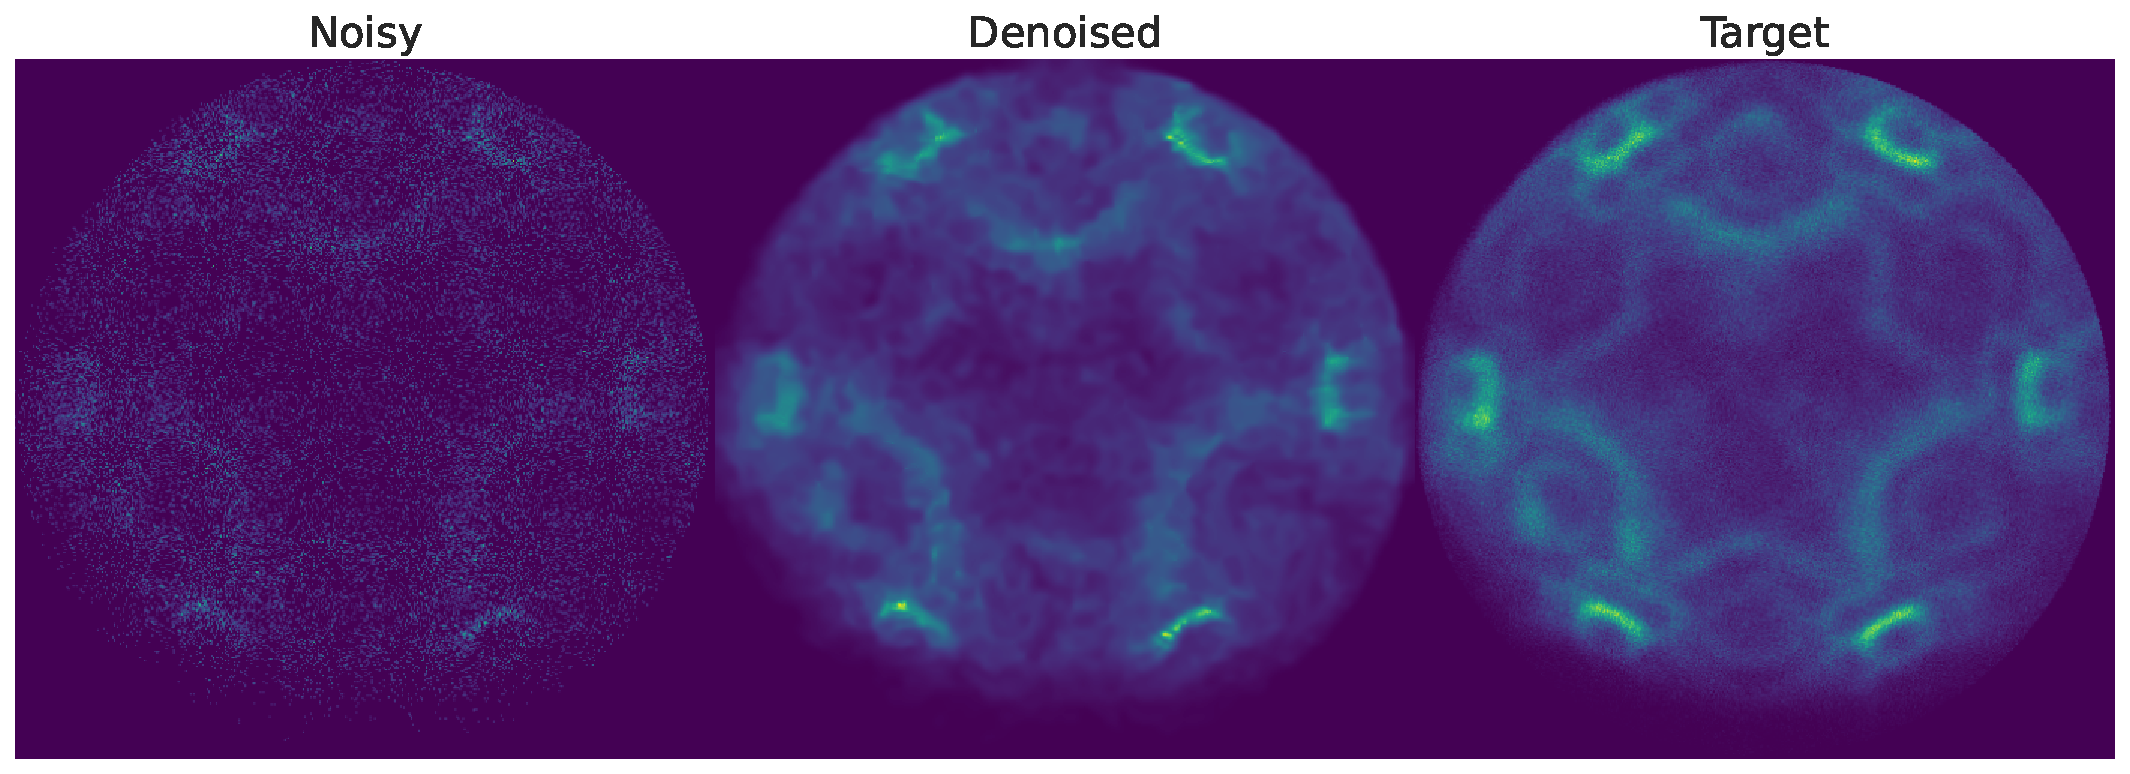
\includegraphics[width=1\linewidth]{images/noisy_denoised_ref_16M_avg_bm3d.pdf}
    \caption{Noisy, denoised, and target images. The noisy and target images are window-averaged with size $w=5$ and $w=15$ along the $E$ dimension, respectively.}
    \label{fig:noisy-denoised-ref-16M-avg-bm3d}
\end{figure}

The above-mentioned evaluation is then repeated by varying $w = \numlist{1;5;10;15}$ for both noisy and target images. \cref{fig:confusion_matrix_msssim_window_avg} presents a confusion matrix that shows how the metric varies when $w$ is varied. It becomes evident that a larger $w$ yields a better comparison for denoising. This is because a larger $w$ reduces the noise in the target image, leading to a more accurate evaluation.

\begin{figure}
    \centering
    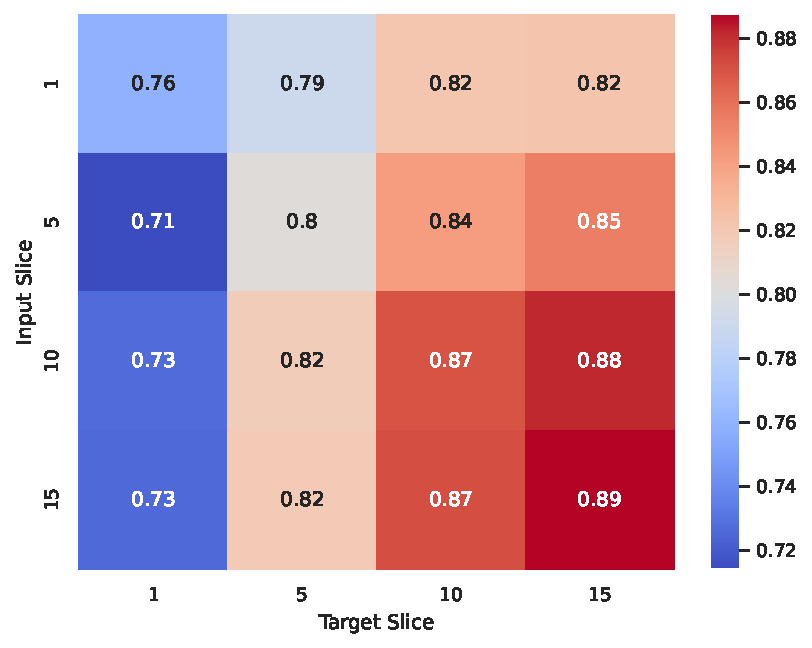
\includegraphics[width=0.5\linewidth]{images/confusion_matrix_msssim_window_avg.pdf}
    \caption{Confusion matrix showing the \gls{MSSSIM} values with different windows $w$ for input and target images. The \gls{MSSSIM} is computed for the denoised images using the Anscombe-BM3D scheme. The matrix shows that using a larger $w$ for target image leads to better comparison of denoising.}
    \label{fig:confusion_matrix_msssim_window_avg}
\end{figure}

\subsection{Finding the Optimal Sigma}
\begin{figure}
    \centering
    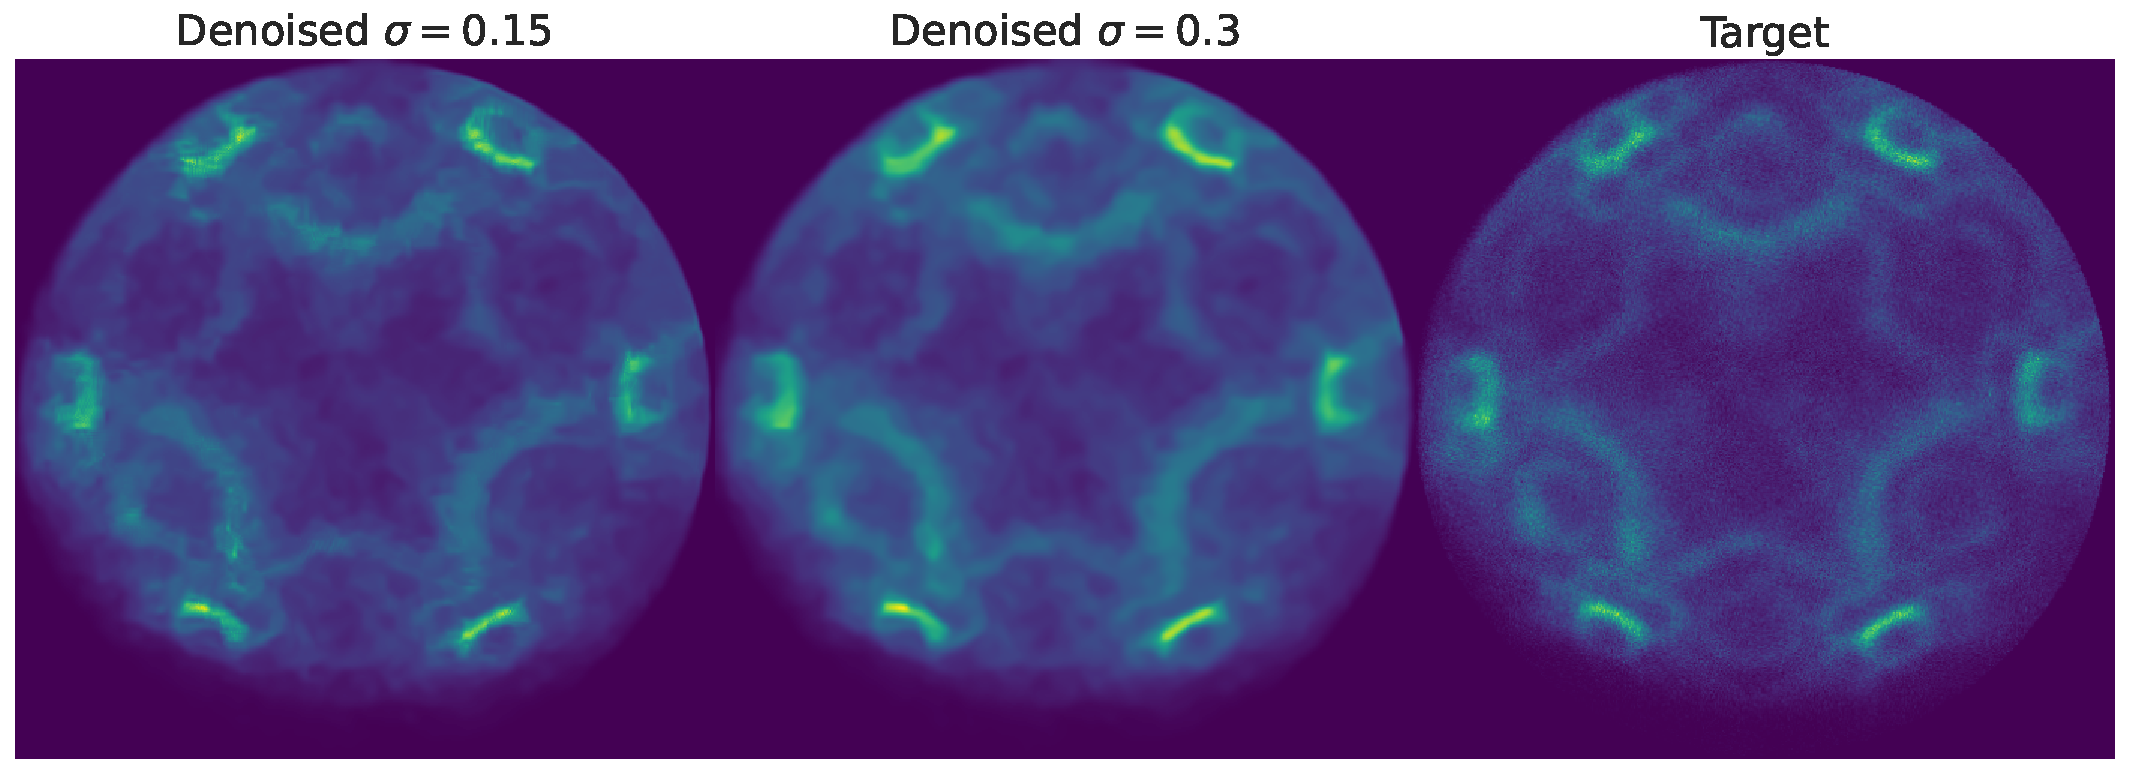
\includegraphics[width=1\linewidth]{images/denoised_optimal_sigma.pdf}
    \caption{Denoised image using the optimal $\sigma_{\text{oo}}=0.15$ (optimal value found for \num{1.6e7} counts from the hyperparameter search) denoised image with $\sigma_{\text{o}}=0.3$ (adjusted optimal value) and the target image.}
    \label{fig:denoised-optimal-sigma}
\end{figure}
Till now, we only focused on a single \gls{ncounts} and applied denoising with a single $\sigma$ value. However, considering that the noise decreases with increased electron counts, we would expect the required level of denoising to decrease i.e. $\gls{ncounts}\propto\frac{1}{\sigma}$.

One way to find the optimal denoising strength would be to estimate the noise level and use that estimate as the $\sigma$ for denoising. A different approach would be to perform a constrained optimization to find optimal $\sigma$ denoted $\sigma_{\text{oo}}$, such that the metric \gls{MSSSIM} is maximized. For user defined parameters to an algorithm, this sort of optimization is known as a hyperparameter search. An exhaustive grid search is the simplest method, but it is computationally expensive. Therefore, we use \texttt{optuna}\footnote{\href{https://optuna.org/}{https://optuna.org/} see citation in acknowledgments.}, which performs Bayesian optimization to find the optimal parameters, optimizing for \num{50} trials.

The search is conducted on a small set of \num{2} identical featured images, featuring the same characteristics as shown in \cref{fig:noisy-denoised-ref-16M-avg-bm3d}, using a window size of ($\gls{winsize} = \num{10}$) across the count range of \numrange{1e6}{4.8e7}. The values of $\sigma$ are constrained between \numrange{0}{5} to prevent the disappearance of features, as higher values can lead to significant loss of detail. The results in \cref{fig:hyperparameter-averaged-10-images} corroborate the hypothesis that the optimal $\sigma$ for denoising decreases with increasing electron counts, a linearly decreasing trend.

\begin{figure}
    \centering
    % First subfigure (Hyperparameter Search with Averaged 10 Images using MS-SSIM)
    \begin{subfigure}[t]{0.49\linewidth}
        \centering
        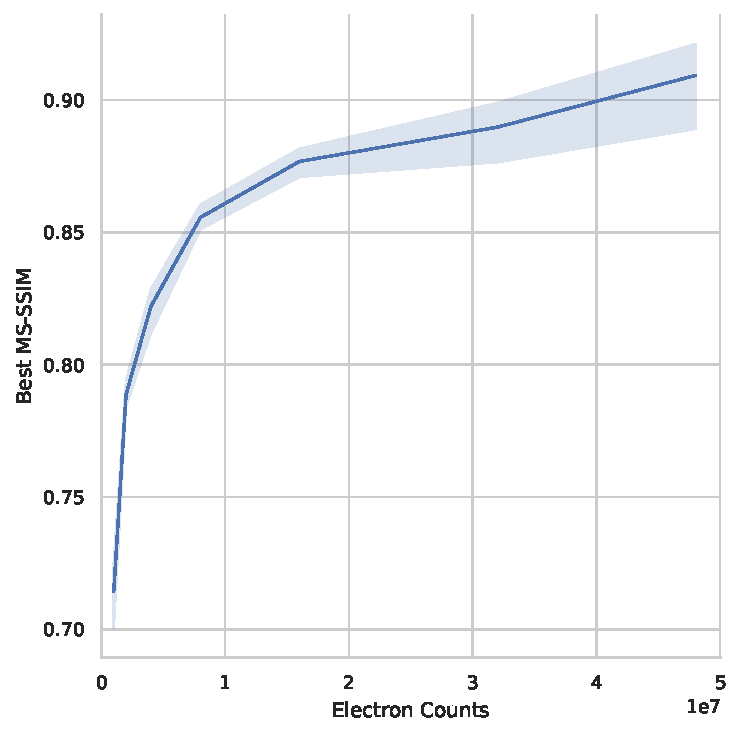
\includegraphics[width=\linewidth]{images/hyperparameter_msssim_averaged_10_images.pdf}
        \caption{Hyperparameter search results using MS-SSIM metric, averaged over 10 images.}
        \label{fig:hyperparameter-msssim-averaged-10-images}
    \end{subfigure}
    \hfill
    % Second subfigure (Hyperparameter Search with Averaged 10 Images using Sigma)
    \begin{subfigure}[t]{0.49\linewidth}
        \centering
        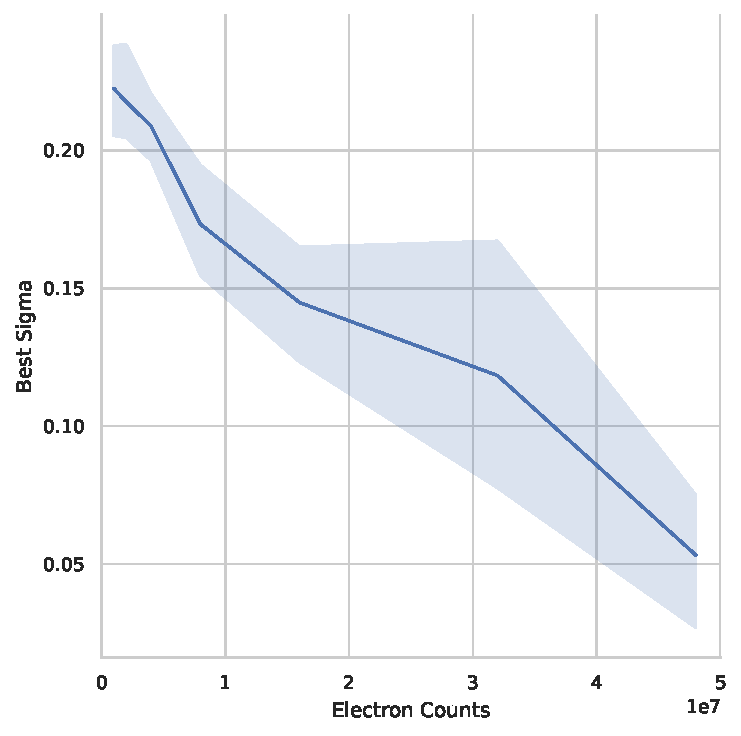
\includegraphics[width=\linewidth]{images/hyperparameter_sigma_averaged_10_images.pdf}
        \caption{Hyperparameter search results using Sigma metric, averaged over 10 images.}
        \label{fig:hyperparameter-sigma-averaged-10-images}
    \end{subfigure}
    \caption{Results of hyperparameter search for \gls{BM3D} $\sigma$ for different electron counts, using the \gls{MSSSIM} metric. The images are window-averaged with $w=10$ from the 3D volume.}
    \label{fig:hyperparameter-averaged-10-images}
\end{figure}

While using \gls{MSSSIM} as the objective function for optimization is good at showing the denoising performance improvement, it leads to more cautious results (low $\sigma_{\text{oo}}$ values) as those fare better against the target, which has the relevant features but is also noisy. To counter that, we scale the optimum $\sigma_{\text{oo}}$ values by a factor of 2 to get a more aggressive denoising and denote that as $\sigma_{\text{o}}$ and use this for denoising. A comparison of the denoised image using the adjusted optimal $\sigma_{\text{o}}$ and the optimal $\sigma_{\text{oo}}$ is shown in \cref{fig:denoised-optimal-sigma}.

The denoising performance below \num{4e6} is poor, with or without the optimal value $\sigma_{\text{oo}}$, even though the \gls{MSSSIM} reports high values. \cref{fig:noisy-denoised-ref-2M-avg-bm3d} and \cref{fig:noisy-denoised-ref-4M-avg-bm3d} show the denoised images for \num{2e6} and \num{4e6} counts, with an average count of \num{0.14} and \num{0.27} in the noisy image, respectively, whereas the average count in target image is \num{12.9}. It can be seen that the perpetual quality of the denoised images is poor, with the features not being well-preserved. This highlights that \gls{BM3D} is not well suited for denoising such low-count images.

\begin{figure}
    \centering

    \begin{subfigure}[b]{1\linewidth}
        \centering
        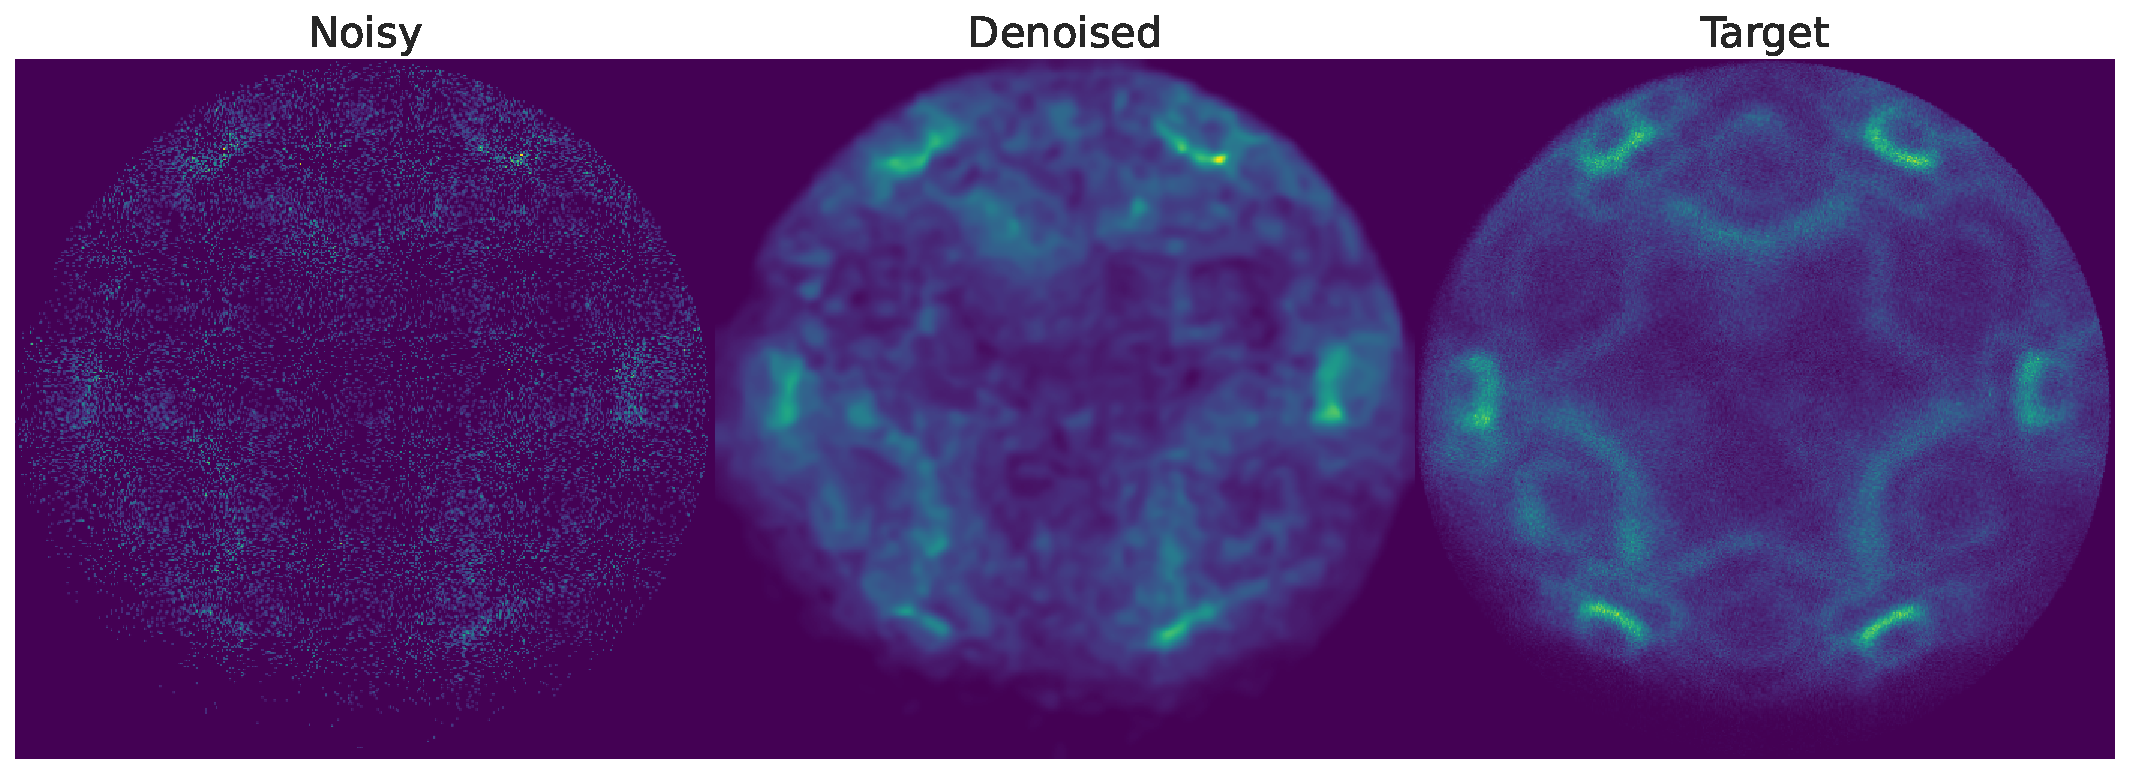
\includegraphics[width=1\linewidth]{images/noisy_denoised_ref_2M_avg_bm3d.pdf}
        \caption{Dataset with $\gls{ncounts}=\num{2e6}$. The denoising performance is quite poor, even with the adjusted optimal $\sigma_{\text{o}}\approx0.4$.}
        \label{fig:noisy-denoised-ref-2M-avg-bm3d}
    \end{subfigure}

    \begin{subfigure}[b]{1\linewidth}
        \centering
        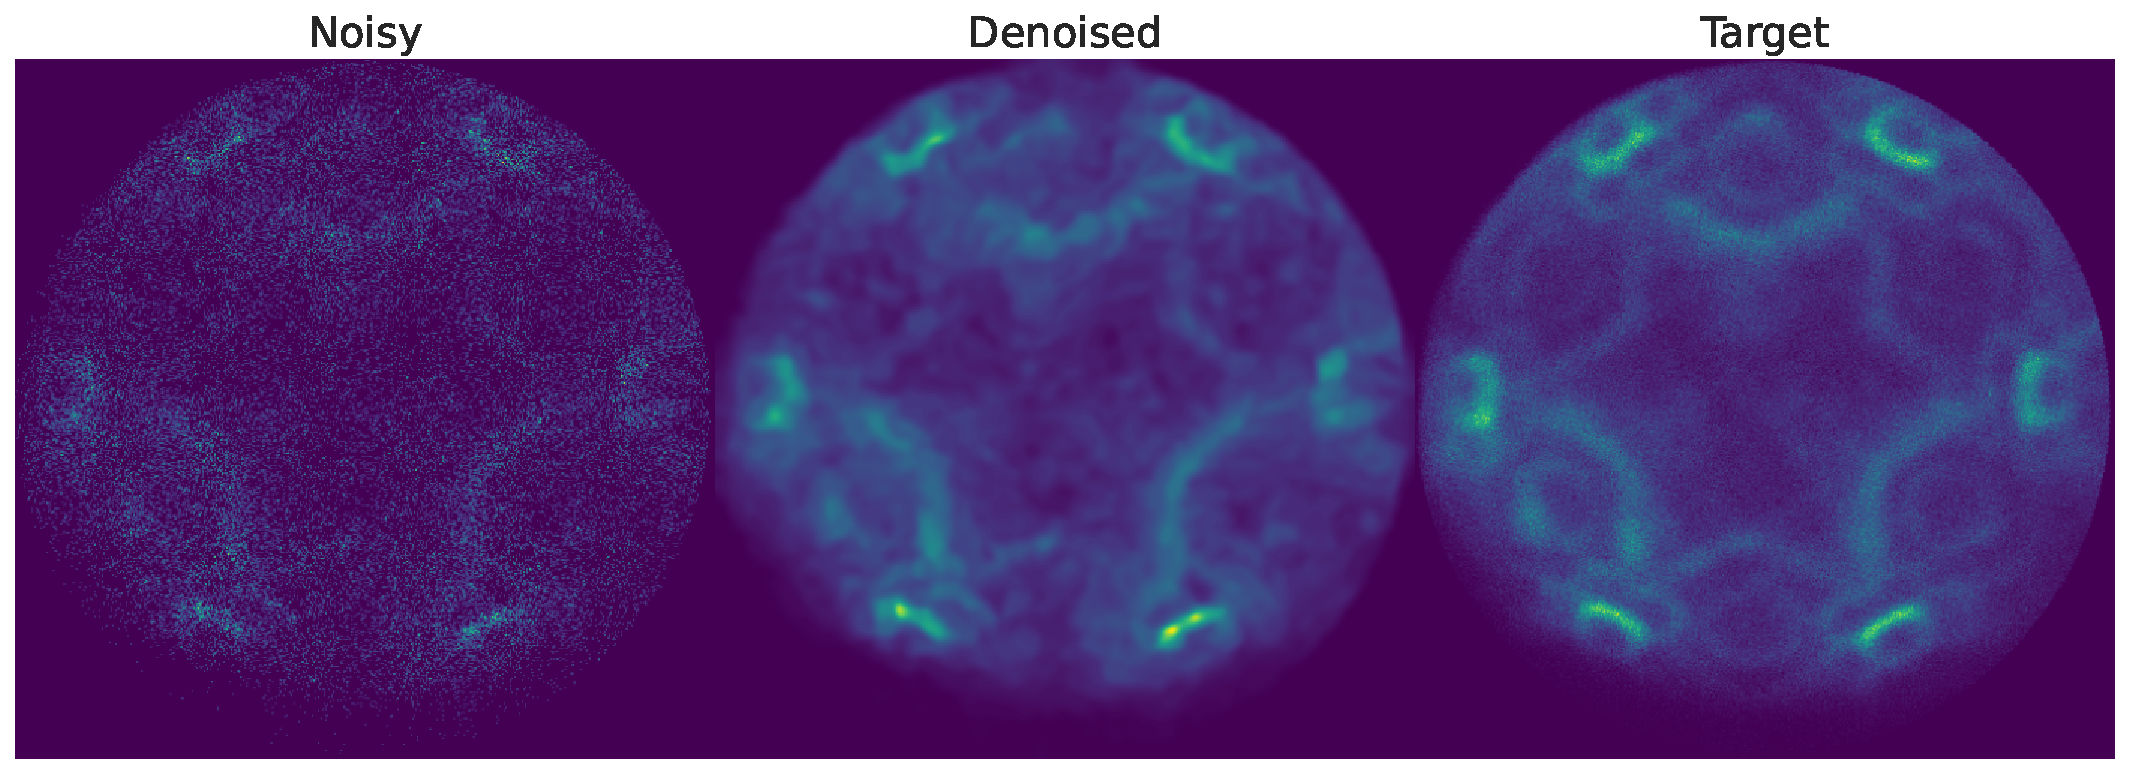
\includegraphics[width=1\linewidth]{images/noisy_denoised_ref_4M_avg_bm3d.pdf}
        \caption{Dataset with $\gls{ncounts}=\num{4e6}$. The denoising performance leaves room for improvement, using the adjusted optimal $\sigma_{\text{o}}\approx0.4$.}
        \label{fig:noisy-denoised-ref-4M-avg-bm3d}
    \end{subfigure}

    \begin{subfigure}[b]{1\linewidth}
        \centering
        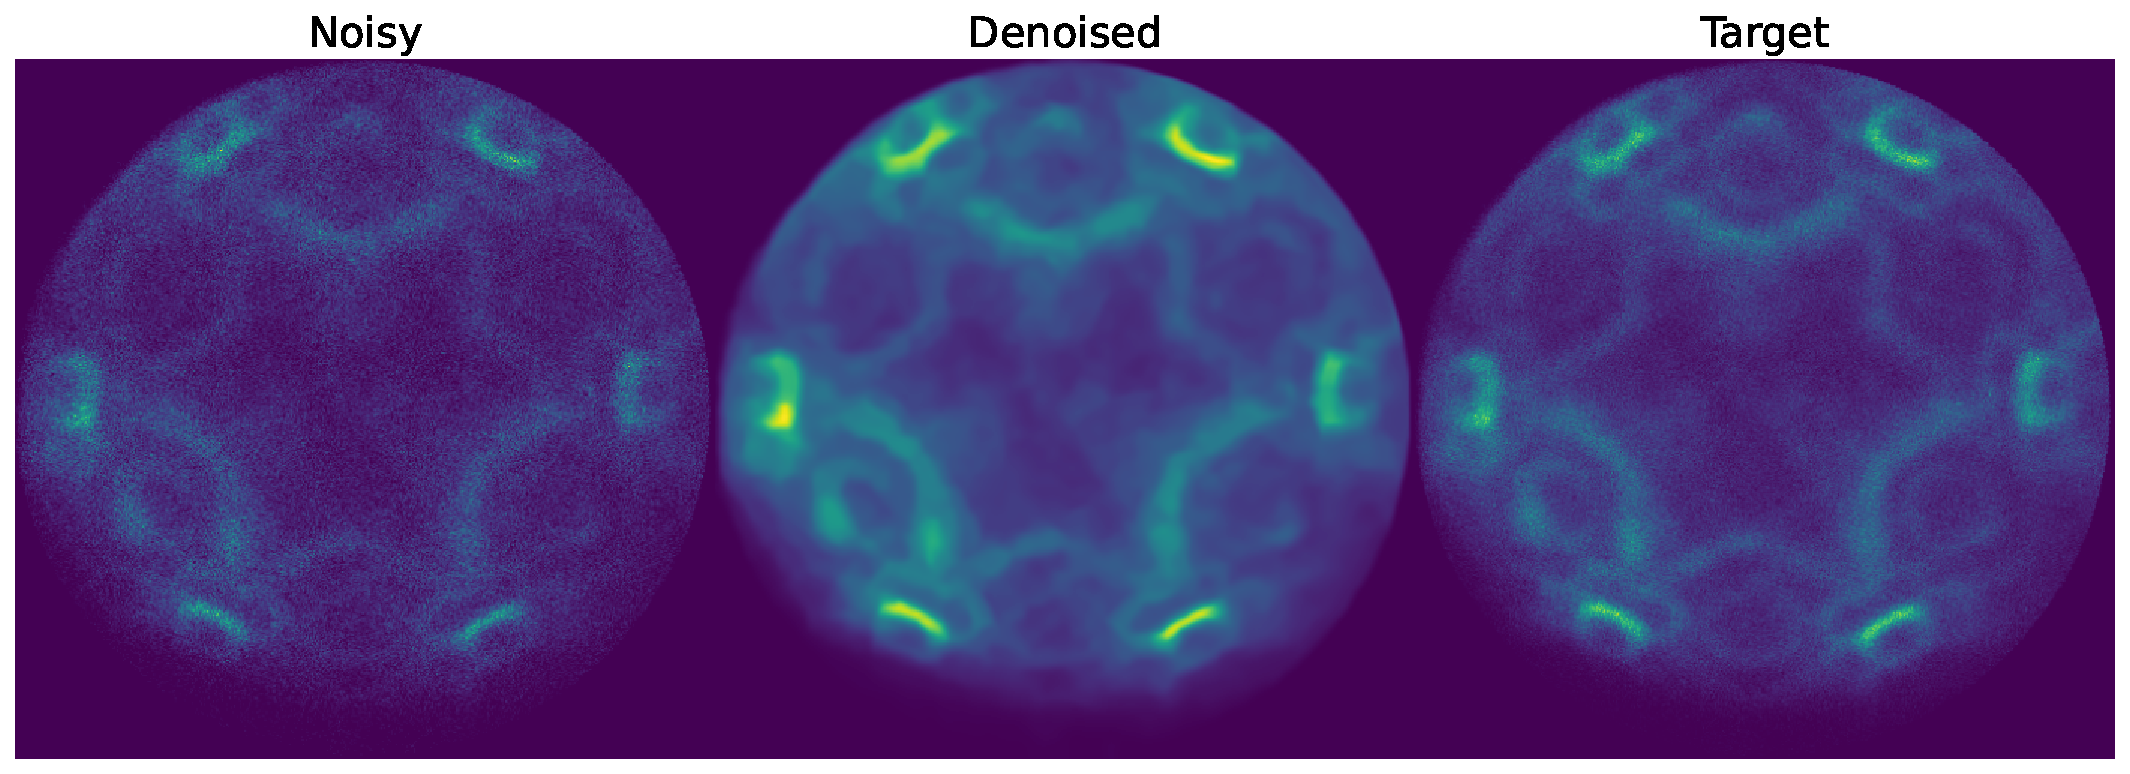
\includegraphics[width=1\linewidth]{images/noisy_denoised_ref_48M_avg_bm3d.pdf}
        \caption{Dataset with $\gls{ncounts}=\num{4.8e7}$. At this \gls{ncounts}, \gls{MSSSIM} reports lower values for the denoised images compared to the noisy images, even though the denoised image features are well-preserved.}
        \label{fig:noisy-denoised-ref-48M-avg-bm3d}
    \end{subfigure}

    \caption{Comparison of noisy, denoised, and target images for $\gls{ncounts}=$\numlist{2e6;4e6;4.8e7}, where the noisy and target images were formed using with $\gls{winsize}=\num{10}$ over \gls{E} to form \gls{kx}-\gls{ky} images. The \gls{BM3D} algorithm with Anscombe transform was used for denoising.}
    \label{fig:combined-noisy-denoised}
\end{figure}

\subsection{Varying Total Counts}
We now evaluate the denoising performance of \cref{alg:bm3d} (\gls{BM3D} without Anscombe) and \cref{alg:anscombe-bm3d} (\gls{BM3D} with Anscombe), using the optimal $\sigma_{\text{o}}$ values determined through the hyperparameter search. A total of \num{1847} images were extracted from two separate noisy realizations of $\gls{ncounts}=\numlist{1e6;2e6;4e6;8e6;1.6e7;3.2e7;4.8e7}$. These are window-averaged with $\gls{winsize}=10$ for both the noisy and target images. 

As before, the \gls{MSSSIM} metric is used, with the baseline computed using the noisy images. Averaging over the large amount of images at varied counts gives us a robust estimate of the denoising performance. Using statistical bootstrapping, where the estimate is computed over multiple resamples of the data, we can also estimate the \num{95}\% confidence interval of the \gls{MSSSIM} metric.

As shown in \cref{fig:bm3d-msssim}, there is a noticeable improvement in image quality with counts up to $\gls{ncounts}=\num{4e7}$, with \gls{MSSSIM} values increasing from \num{0.6} to \num{0.83}. Beyond this count, the metric starts reporting lower values for denoised results, whereas visual inspection reveals that the denoised images contain similar information as the target, smoother with preserved features. We can see this in \cref{fig:noisy-denoised-ref-48M-avg-bm3d}, where the denoised image has a lower \gls{MSSSIM} value compared to the noisy image, but the features are well-preserved. This necessitates the need for higher quality target images for better evaluation.

\begin{figure}
    \centering
    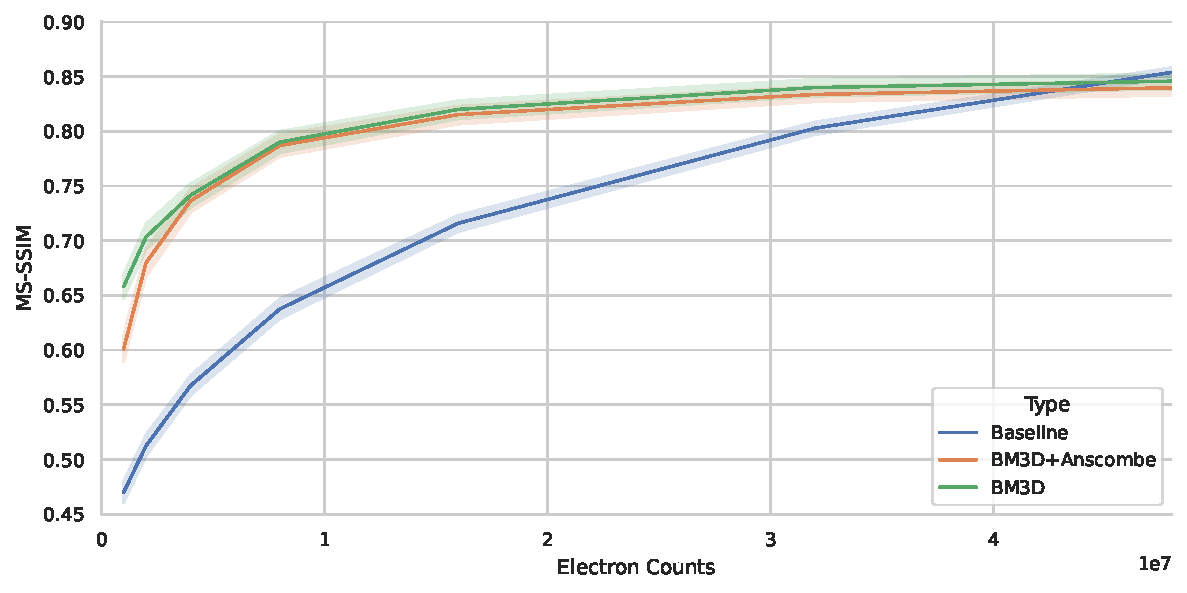
\includegraphics[width=1\linewidth]{images/bm3d_msssim.pdf}
    \caption{Denoising performance of the \gls{BM3D} algorithm, with and without the Anscombe transformation. The optimal $\sigma_{\text{o}}$ values determined through the hyperparameter search are used. The images are window-averaged with $\gls{winsize}=10$ slices for both the noisy and target images. The baseline metric is computed using the noisy image as input.}
    \label{fig:bm3d-msssim}
\end{figure}


The most notable finding is that the application of the \gls{VST} leads to a slightly worse performance (\cref{fig:bm3d-msssim} orange vs. green lines), despite the expectation that it would enhance denoising performance for Poissonian noise. In previous work by \citeauthor{makitaloOptimalInversionAnscombe2011}, the authors demonstrated that applying the Anscombe transform indeed improves denoising performance. This strongly suggests that the noise statistics in the image deviate from a Poisson distribution. One reason is the window-averaging used to form the images, that might have altered the noise statistics. The other obvious reason is that the electron count statistics forming the images are not Poissonian. This shall be the topic of the next chapter. 
